\documentclass[12pt]{article}

\usepackage{a4wide}
\usepackage[utf8]{inputenc}

\usepackage{graphicx}
%\usepackage{palatino}

%\pagestyle{empty}

\parindent=0pt
\begin{document}

\section{Computing Moments and Features}

Moments are common features that are used in object classification since they are easy to compute.

The moment that is related to the coordinate system is computed as follows

\begin{equation}
m_{p, q} = \sum\limits_{x} \sum\limits_{y} x^p y^q f(x, y) \, ,
\end{equation}
(in our case, we do not have to multiply the coordinates by the corresponding image function, since it is almost the same).
\\
\\
Let us explain some important moments:
\\
\\
The \textbf{area} of an object can be computed as $m_{0, 0}$.
\\
\\
The \textbf{center of the mass} of an object:
\begin{equation}
x_t = \frac{m_{1, 0}}{m_{0, 0}}, \quad y_t = \frac{m_{0, 1}}{m_{0, 0}}
\end{equation}

The \textbf{perimeter} of an object may be computed using a simple algorithm that scans each pixel of the object and if the four neighbour of the pixel
contains the same values as the central pixel than this pixel does not contribute to the perimeter, otherwise it does.

%The \textbf{perimeter} of an object may be computed using a simple algorithm that scans each pixel of the object and if the four neighbour of the pixel
%contains the same values as the central pixel than this pixel does not contribute to the perimeter, otherwise it does.

The moment that is related to the center of the mass of an object is computed as follows

\begin{equation}
\mu_{p, q} = \sum\limits_{x} \sum\limits_{y} (x - x_t)^p (y - y_t)^q f(x, y) \, ,
\end{equation}
(in our case, we do not have to multiply the coordinates by the corresponding image function, since it is almost the same).

\subsection{Features for our Classification}

We'll use two features to describe objects in our images. Let us call them $F_1$ and $F_2$. They can be described as follows

\begin{equation}
    F_1 = \frac{\mathrm{Perimeter}^2}{100 \mathrm{Area}}, \quad \mathrm{Area} = \mu_{0,0}
\end{equation}

\begin{equation}
    F_2 = \frac{\mu_{\mathrm{min}}}{\mu_{\mathrm{max}}},
\end{equation}
where $\mu_{\mathrm{min}}, \mu_{\mathrm{max}}$ are

\begin{equation}
    \begin{array}{c}
    \mu_{\mathrm{max}} \\
    \mu_{\mathrm{min}}
    \end{array}
    = \frac{1}{2} \left( \mu_{2,0} + \mu_{0,2} \right) \pm \frac{1}{2} \sqrt{ 4 \mu_{1,1}^{2} + \left( \mu_{2,0} - \mu_{0,2} \right)^2 }.
\end{equation}

\begin{figure}[hb]
\begin{centering}
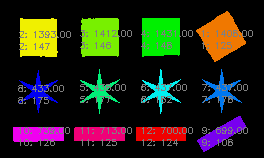
\includegraphics[width=0.4\textwidth]{areas_and_perimeters.png}
\caption{An example of computer areas and perimeters for each object. The \textit{first} row represents area, the \textit{second} row represents perimeter. }
\end{centering}
\label{fig:areas_and_perimeters}
\end{figure}

\end{document}

